% !TeX encoding = UTF-8
% !TeX program = xelatex
% !TeX spellcheck = fr
% !TeX root = tm_astro_main.tex

\chapterFormat
\chapter{Supernovas}\label{3}

Les étoiles dépassant 9 $M_\odot$ produisent obligatoirement une supernova au terme de leur vie (§\ref{2}). Ces explosions, qui peuvent atteindre des luminosités équivalentes à 1 milliard de soleils, éjectent leur matière à quelques fractions de la vitesse de la lumière. En effet, la supernova relâche une quantité d'énergie, sous forme cinétique, égale à 1 Bethe. 1 Bethe correspond à $10^{44}$J; cette unité a été nommée en l'honneur de Hans Bethe pour ses travaux sur les supernovas. A titre de comparaison, la bombe Tsar, plus puissante bombe nucléaire jamais utilisée, dégagea une énergie de $10^{17}$J, ce qui est $10^{27}$ fois moins fort que l'énergie cinétique d'une supernova. Cependant, toutes les supernovas ne sont pas causées par l'effondrement gravitationnel d'une étoile massive (§\ref{2}), il existe d'autres processus qui permettent d'aboutir à de telles explosions.

\section{Types de supernovas}\label{3.1} 

Les supernovas ont été historiquement classées selon leur spectre électromagnétique. Si l'on détecte de l'hydrogène dans l'explosion, alors la supernova est de type II. A l'opposé, si l'on n'en détecte pas, alors la supernova est de type I. Cependant, cette classification ne tient pas compte de l'origine du phénomène, c'est pourquoi des subdivisions supplémentaires ont été créées afin de tenir compte d'autres critères. Les supernovas résultant d'un effondrement gravitationnel d'une étoile massive sont appelées supernovas à effondrement de cœur et sont classées dans les type Ib, Ic et II (§\ref{3.1.1}). Le groupe Ia correspond aux supernovas appelées thermonucléaires. Ces dernières sont causées par une naine blanche accrétant de la matière à une étoile proche (§\ref{3.1.2}).

\subsection{Supernovas à effondrement gravitationnel}\label{3.1.1} 

Les supernovas à effondrement gravitationnel marquent la fin de vie des étoiles dont la masse est supérieure à 9 $M_\odot$. Ces étoiles possèdent un noyau en fer, entouré par des couches de différentes compositions (Fig. \ref{Fig. 2.6}). Comme plus aucune réaction nucléaire n'a lieu dans le cœur (§\ref{2.4}), celui-ci commence donc à se contracter. Seul la pression de dégénérescence permet de freiner cette contraction, seulement, lorsque le noyau dégénéré dépasse la masse de Chandrasekhar (1,46 $M_\odot$), le cœur poursuit sa contraction. Du fait que le gaz est dégénéré, la température peut monter extrêmement rapidement sans occasionner des changements de pression. A partir de $10^{9}$K, la température est suffisante pour déclencher la photodésintégration du fer (Eq.  \ref{Eq. 3.1}).  % note de bas de page sur temp min/max %

\begin{equation} \ce{\ce{^{56}Fe} -> \ce{13\ce{^{4}He}} + \ce{4n} - {124MeV}}\label{Eq. 3.1}\end{equation}\smallskip

Cette réaction hautement endothermique, favorisant la contraction du cœur, décompose le fer en hélium et en neutrons. De plus, les photons, de plus en plus énergétiques sous l'effet de la pression, deviennent capable de briser l'hélium en protons et en neutrons. La pression devient telle que les électrons sont capturés par les protons dans un processus qui s'appelle la neutronisation (Eq. \ref{Eq. 3.2}).

\begin{equation} \ce{p + e{^-} -> n + $\nu$\label{Eq. 3.2}}\end{equation}\smallskip

Ce processus diminue le nombre d'électrons et par extension, la pression de dégénérescence des électrons; l'effondrement est encore une fois favorisé. Comme il ne reste bientôt plus que des neutrons, de manière analogue aux électrons, une pression de dégénérescence liée aux neutrons se créée. Cette-fois ci, la contraction  peut être stoppée. La force nucléaire forte, qui lie les protons et les neutrons dans le noyau atomique, devient répulsive lorsque la pression est supérieure à la densité d'un noyau atomique, qui est de l'ordre de $10^{17}$ kg  m$^{-3}$. Ainsi, une énorme onde de choc est crée par les couches supérieures de l'étoile lorsqu'elles rebondissent contre le noyau qui est devenu répulsif.
Les neutrinos créés lors de la neutronisation, environ $10^{57}$, emportent 99\% de l'énergie de l'explosion; les 1\% restants sont répartis entre l'énergie cinétique de la matière expulsée (0,9\%) et la luminosité de l'explosion (0,1\%). Ces particules très énergétiques possèdent une masse quasiment nulle et voyagent à des vitesses proches de celle de la lumière, en plus de cela, elles n'interagissent presque pas avec la matière. Seulement, vu leur nombre élevé ($10^{57}$), une partie d'entre-eux vont chauffer les couches de l'étoile lors de leur expulsion. Aujourd'hui, nous pensons que les neutrinos sont les principaux responsables de l'explosion de la supernova.\smallskip

Les supernovas de type Ib, Ic et II se déroulent toutes selon le processus vu ci-dessus. Ce qui les différencie, c'est leur spectre ainsi que leur courbe de lumière\footnotemark[1] (Fig. \ref{Fig. 3.1}).\bigskip

\begin{itemize}
	
	\item Type Ib: Premièrement, il se caractérise par une absence d'hydrogène dans son spectre électromagnétique, ce qui fait de lui une supernova de type I. En plus de cela, nous retrouvons de l'hélium dans sa composition. Sa courbe de lumière montre un taux de décroissance inférieure aux supernovas de type IIL (voir Type II).
	
	\item Type Ic: Comme le type Ib, il ne possède pas d'hydrogène dans son spectre. Cependant, nous ne trouvons non plus pas d'hélium. La raison pour laquelle l'hydrogène ou l'hélium ne font pas partie du spectre électromagnétique des types Ib et Ic est soit que l'étoile a été balayée par de forts vents stellaires, soit qu'il s'est produit un transfert de matière dans un système binaire. Pour finir, les types Ib et Ic possèdent la même courbe de lumière.
	
	\item Type II: Le type II se distingue de tout les autres grâce à la présence d'hydrogène dans son spectre électromagnétique. Lors d'observations de supernovas composées notamment d'hydrogène, on a remarqué que deux courbes de lumière bien distinctes se délimitaient. C'est pourquoi les supernovas de type II sont encore séparées en type IIL(L pour linéaire) et IIP (P pour plateau). La courbe de lumière du type IIP forme un plateau dans les premiers mois suivants la supernova, tandis que la luminosité du type IIL décroît presque linéairement.
	
\end{itemize}

\begin{figure}[H]
	\centering
	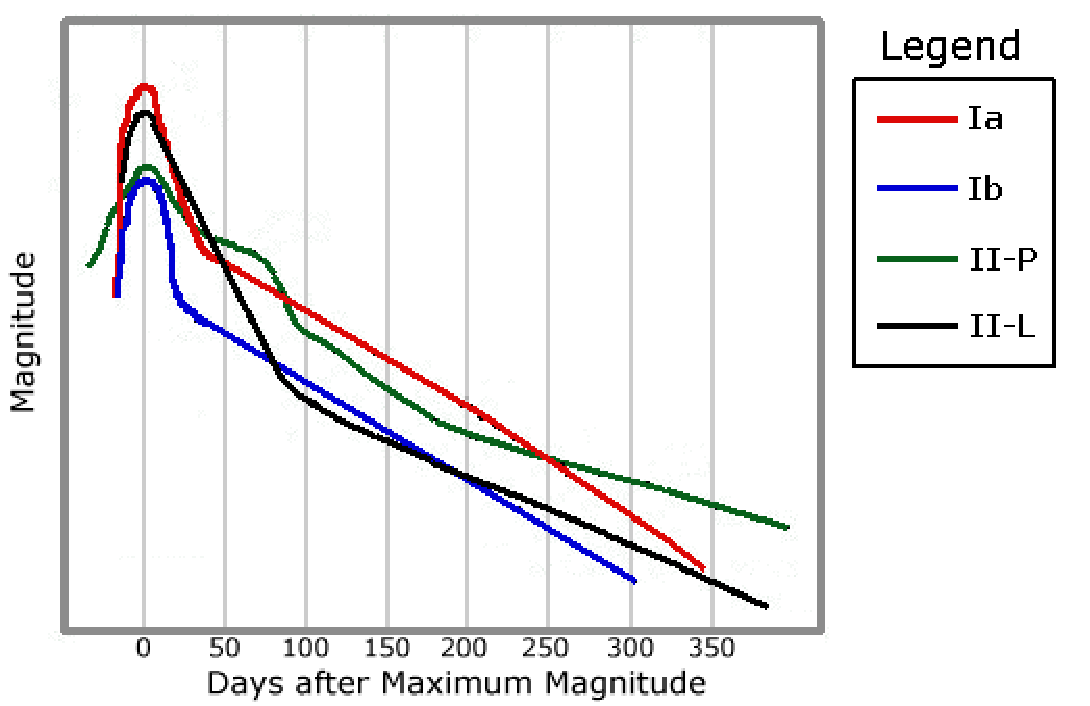
\includegraphics[scale=0.33]{images/lightcurves}
	\caption[Comparaison des courbes de lumière théoriques des différents types de supernovas \label{Fig. 3.1}\newline \url{http://www.talkorigins.org/faqs/supernova/}]{Comparaison des courbes de lumière théoriques des différents types de supernovas \label{Fig. 3.1}}
	\label{Fig. 3.1}
\end{figure}

\vfill
\footnotetext[1]{Une courbe de lumière est un graphique représentant l'évolution temporelle de la luminosité d'un astre.}

\subsection{Supernovas thermonucléaires}\label{3.1.2} 

Les supernovas thermonucléaires nécessitent un système composé d'au moins deux étoiles. Parmi ces étoiles, l'une d'entre elle doit être une naine blanche tandis que l'autre doit se situer sur la fin de la séquence principale. Pour qu'un transfert de matière puisse s'opérer, il faut que la compagne de la naine blanche franchisse son lobe de Roche. Un lobe de Roche est le volume critique autour d'une étoile dans lequel la matière reste en orbite autour de celle-ci, dépassé cette limite la matière quitte son orbite. De plus, il n'y a pas que la force gravitationnelle qui est prise en compte dans le calcul du lobe, la force centripète associée au système binaire l'est aussi. Si l'on projette les deux lobes sur un plan, ils forment une sorte de huit. Lorsque les couches supérieures de la géante dépassent la surface limite, il peut y avoir transfert de matière entre les étoiles. Cependant, la matière ne transite pas d'une étoile à l'autre par n'importe quel chemin, elle passe par l'intersection entre les deux lobes de Roche, le centre du huit (Fig. \ref{Fig. 3.2}).\bigskip

\begin{figure}[H]
	\centering
	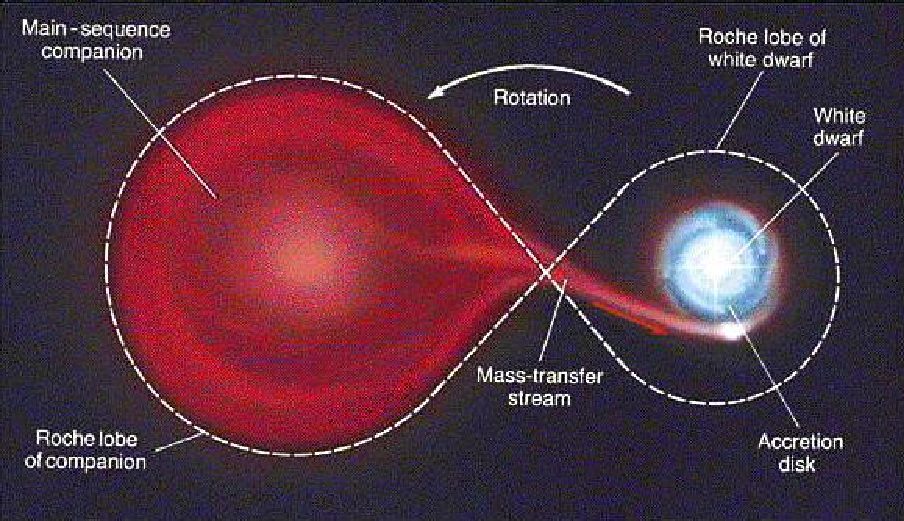
\includegraphics[scale=0.6]{images/lobederoche}
	\caption[Transfert de matière dans un système binaire et lobes de Roche\newline \url{http://chandra.harvard.edu/edu/formal/snr/bg3.html}]{Transfert de matière dans un système binaire et lobes de Roche}
	\label{Fig. 3.2}
\end{figure}\bigskip 

De plus en plus de matière commence donc à orbiter autour de la naine blanche, ce qui forme un disque d'accrétion autour de celle-ci. Ce disque, augmentant de masse, a pour effet d'accroître la pression et la température de l'étoile. Juste avant que la naine blanche n'atteigne la masse de Chandrasekhar (1,44 $M_\odot$) 
 , le carbone ainsi que l'oxygène se mettent à fusionner, chacun indépendamment, de manière anarchique. Comme le gaz composant l'étoile est dégénéré, la température peut donc croître extrêmement rapidement (§\ref{3.1.1}). L'augmentation de température accélère la fusion chaotique de l'oxygène et du carbone. Par un phénomène encore mal compris et sujet à débat, l'étoile explose sous l'effet d'un ultime emballement des fusions thermonucléaires. Plus aucun noyau de subsiste après cette explosion, toute la matière s'éparpille dans le milieu interstellaire.\smallskip
 
 Les supernovas de type Ia sont les seules supernovas thermonucléaires. Cependant, comme les types Ib et Ic, elles ne possèdent pas d'hydrogène dans leur spectre électromagnétique, néanmoins, contrairement à eux, on distingue la présence de raies de silicium dans leur composition. 
 
 \section{Nucléosynthèse lors d'une supernova}\label{3.2} 
 
 L'explosion d'une supernova permet de créer des éléments plus lourds que ceux produits lors de la nucléosynthèse stellaire standard. Lors d'une supernova, un important flux de neutrons (10$^{20}$ neutrons cm$^{-2}$ s$^{-1}$) balaie les couches supérieures de l'étoile. Ces neutrons, ne possédant pas de charge électrique, peuvent être capturés par des atomes avoisinants grâce aux exceptionnelles conditions de pression et de température (T=10$^{9}$K et P=10$^{9}$ g cm$^{-3}$); ce phénomène s'appelle la capture de neutrons rapide, ou processus r\footnotemark[2]. 
 Plus un atome capte des neutrons, plus il deviendra un grand isotope. Le processus r s'arrête soit lorsque le noyau remplit toutes ses couches nucléaires et devient donc extrêmement stable, soit parce que le noyau est trop instable et est soumis à la radioactivité $\beta^{-}$.\smallskip
 
 Le noyau, lorsqu'il remplit toutes ses couches nucléaires, devient moins sensible aux réactions nucléaires. Remplir ses couches nucléaires signifient atteindre un nombre de nucléons égale à 20,28,50 ou encore 126. Ces nombres déterminé expérimentalement, pour lesquels un noyau atomique est très stable, sont aussi appelés nombres magiques.\smallskip 
 
 Si l'isotope devient instable, alors un neutron se dégrade en un proton, un électron et un antineutrino  par radioactivité $\beta^{-}$ (Eq. \ref{Eq. 3.3}).
 
\begin{equation} \ce{n -> \ce{p+} + \ce{e-} + $\overline{\nu}$_{e}}\label{Eq. 3.3} \end{equation}\smallskip
 
 Comme le noyau a gagné un proton, un nouvel élément est créé. Grâce à ce processus (Fig. \ref{Fig. 3.3}), des atomes tels que le plomb, l'or ou l'uranium peuvent être créés. Ce cycle peut se répéter tant que les conditions de flux neutronique, de pression et de température à la capture de neutrons sont remplies. Cependant, ces conditions ne sont remplies que pendant quelques secondes lors de l'explosion de la supernova. Tout ces éléments lourds sont par la suite répandus dans le milieu interstellaire à cause de l'explosion (§\ref{5}).
 
 \begin{figure}[H]
 	\centering
 	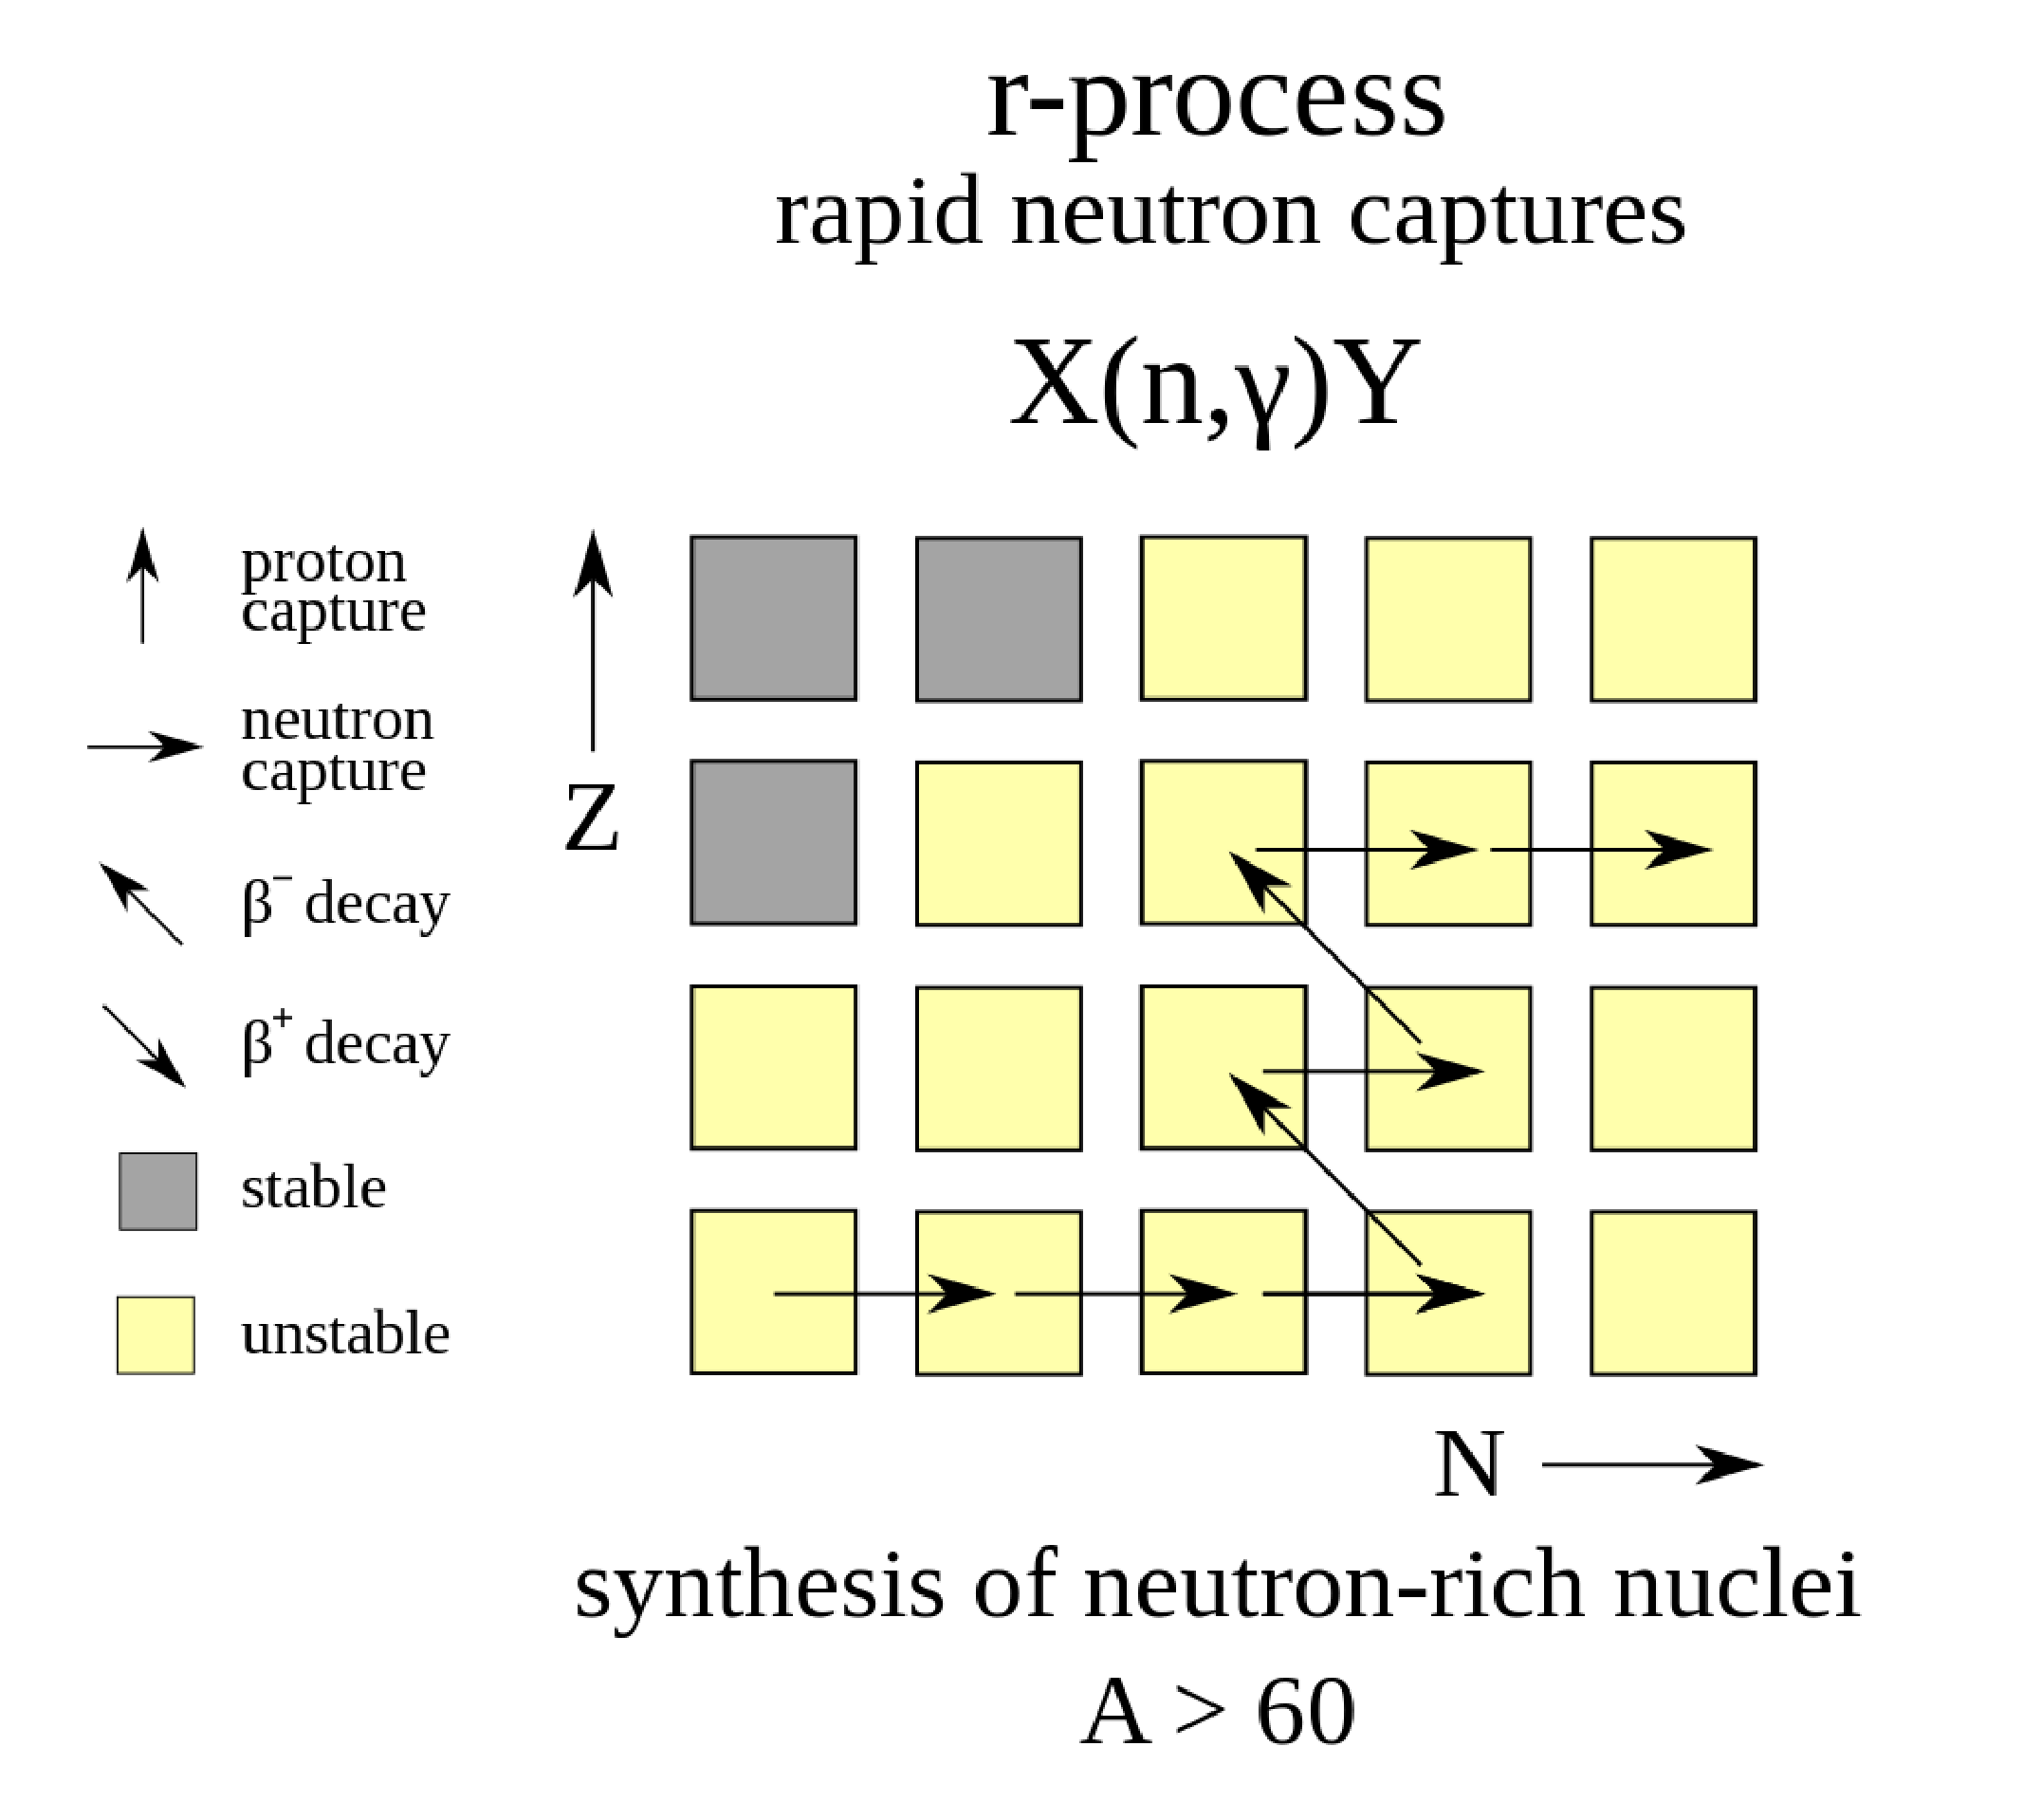
\includegraphics[scale=0.16]{images/processusr}
 	\caption[Trajectoire d'un atome capturant des neutrons dans le tableau périodique des éléments\newline \url{https://it.wikipedia.org/w/index.php?title=Processo_r&oldid=103197986}]{Trajectoire d'un atome capturant des neutrons dans le tableau périodique des éléments}
 	\label{Fig. 3.3}
 \end{figure} 

 \vfill
 \footnotetext[2]{Il existe aussi un processus s (slowly) de capture de neutrons qui prend lieu dans des étoiles AGB (§2.2.2) déjà enrichies par une supernova précédente.}



 
 
